\subsection{Allgemeine Zusammenhänge}
\formTab{Logarithmus zu beliebiger Basis}{\log_b(x) = \frac{\ln(x)}{\ln(b)}}
\formTab{Asymptote $a$ zu $\log_b (x)$ an $(1,0)$}{a=\fracd{1}{\ln(b)}(x-1)}
\formTab{Fourier Transformation}{X(f) = \int\limits_{-\infty}^\infty x(t) \cdot e^{-j2\pi f t}\;dt}

\subsubsection{Fourier Korrespondenzen}
Für reelle $x(t)$ gilt die komplex konjugierte Symmetrie für die Transformierte:
\formTab{Symmetrie}{X(-f) = X^*(f) \quad \land \quad |X(-f)| = |X(f)|}
\begin{align}
	g(t) \cdot T = \lbrace 
		\begin{cases}
		1 & ,\;t = 0\\
		\frac{\sin \left(\frac{\pi t}{T}\right)}{\pi \frac{t}{T}} & ,\;sonst
	\end{cases} \quad &\laplace \quad G(f) = \lbrace 
	\begin{cases}
		1 & ,\; |f| \leq \frac{R_S}{2} = \frac{1}{2T}\\
		0 & ,\; sonst
	\end{cases} \label{eq:fourier_corr_einzelimpuls}\\
	A \quad &\laplace \quad A\cdot 2\pi \delta(w)\\
	A \quad &\laplace \quad A\cdot 2\pi \delta(f)\\
	x(t) \cdot e^{\pm j 2 \pi f_0 t}\quad &\laplace \quad X(f \mp f_0)\\
	x(t) \cdot e^{\pm j 2 \pi w_0 t}\quad &\laplace \quad X(w \mp w_0)\\
	u(t) = \alpha_A \cdot x(t) \cdot \cos(w_o t) \quad &\laplace \quad U(w) = \alpha_A \frac{1}{2} \left[ X(w+w_0) + X(w-w_0)\right]\label{eq:fourier_corr_am_1}\\
	x(t) + A_{off} \quad &\laplace \quad X(w) + 2\pi \cdot A_{off} \cdot \delta(w)\label{eq:fourier_corr_am_off}\\
	V(\omega) = \frac{1}{2} X(\omega) \cdot \cos(\psi)\quad &\laplace \quad v(t) = \frac{1}{2}x(t) \cdot \cos(\psi) \\
	1\quad &\laplace \quad 2 \pi \delta (\omega)\\
	\cos(\omega_{0} t) \quad &\laplace \quad \pi(\delta(\omega - \omega_{0}) + \delta(\omega + \omega_0)) \\
	\sin(\omega_{0} t) \quad &\laplace \quad \frac{\pi}{j}(\delta(\omega - \omega_{0}) - \delta(\omega + \omega_0))\\
	e^{j \omega_0 t} \quad &\laplace \quad 2 \pi \delta(\omega - \omega_0)\\
	x(t) \quad &\laplace \quad X(\omega)\\
	X(t)  \quad &\laplace \quad 2 \pi x^{*} (-\omega) \\
	x(t) \quad &\laplace \quad X(f)\\
	X(f)  \quad &\laplace \quad x^{*} (-\omega) \\
	g(t) = \begin{cases} 
	1 &,\; |t| \leq \frac{T}{2} \\
	0 &,\; sonst
	\end{cases} \quad &\laplace \quad G(f) \cdot R_s = \begin{cases}
	1 & ,\; f=0 \\
	\frac{\sin(\pi \frac{f}{R_s})}{\pi \frac{f}{R_s}} & ,\; sonst
	\end{cases} \\
	g(t) \cdot T = \begin{cases}
	1 & ,\; t  = 0 \\
	\frac{ \sin(\pi \frac{t}{T})}{\pi \frac{t}{T}} & ,\; sonst
	\end{cases} \quad & \laplace \quad G(f) = \begin{cases}
	1 & ,\; |f| \leq \frac{R_s}{2} = \frac{1}{2T} \\
	0 & ,\; sonst
	\end{cases}
\end{align}

\subsection{Wahrscheinlichkeit von Quellensymbolen}
\formTab{Auftrittswahrscheinlichkeit von $x_i$ a)}{P\left[x_i \right]  = P_i  \text{ mit } 0 \leq P_i \leq 1}
\formTab{Auftrittswahrscheinlichkeit von $x_i$ b)}{\sum\limits_{i=1}^N P_i \overset{!}{=} 1}
\formTab{Bedingung für Gleichverteilung]}{P_i \overset{!}{=} \frac{1}{N}}

\subsection{Relative Häufigkeit}
\formTab{Relative Häufigkeit}{h = \frac{\text{Zahl der Treffer}}{\text{Zahl der Versuche}} =  \frac{k_T}{K} \leq 1} 
\formTab{Definition der Wahrscheinlichkeit}{P\left[ \text{Treffer} \right] = \lim\limits_{K\rightarrow \infty} \frac{k_T}{K} = P}

\subsection{Verbundwahrscheinlichkeit}
\formTab{Verbundwahrscheinlichkeit}{P\left[X_A, X_B \right] = P\left[\text{Ereignis A} \cap \text{Ereignis B} \right]}
\formTabL{Multiplikationssatz}{P\left[ X_A, X_B \right] = P\left[ X_A \right] \cdot P\left[ X_B \right]}{grundl_verbund_mult}
\begin{bem}
Der in \eqref{eq:grundl_verbund_mult} genannte Satz gilt nur für statistisch unabhängige Ereignisse, also Ereignisse die sich gegenseitig nicht beeinflussen.
\end{bem}

\subsection{Informationsgehalt}
\formTab{Informationsgehalt}{I(x_i) = \log_2\left(\frac{1}{P_i}\right) \left[ \frac{bit}{Symbol}\right] }

\subsection{Mittlerer Informationsgehalt einer Quelle}
\formTab{Entropie}{H(X) = E\left[I(x_i)\right] = \sum\limits_{i=1}^N P_i \cdot I(x_i) \formTnQQQ = \sum\limits_{i=1}^N P_i \cdot \ld\left(\frac{1}{P_i}\right)}
\formTab{Maximierung}{\max H(X) = H_0 =  \ld (N)}
\begin{bem}
Das Maximum der Entropie wird für gleichförmig verteilte Symbolquellen erreicht, also muss gelten: $0 \leq H(X) \leq \ld(N)$ und $P_i = \frac{1}{N}, \; i=1,...,N$.
\end{bem}

\subsubsection{Mittlerer Informationsfluss}
\formTab{Mittlerer Informationsfluss}{H^* = \fracd{H(X)}{T}}

\subsection{Redundanz einer Quelle}
\formTab{Redundanz}{R(X) = H_0 - H(X) = \ld(N) - H(X)}
\formTabL{Relative Redundanz}{r = \fracd{R(X)}{H_0} = 1 - \fracd{H(X)}{H_0}}{grundl_red_rel}
\begin{bem}
	Die Redundanz wird hauptsächlich durch zwei Methoden beeinflusst. Die Quellencodierung, die Redundanz entfernt und die Kanalcodierung, die Redundanz kontrolliert einfügt. Meist werden beide Verfahren zweistufig kombiniert.
\end{bem}

\subsection{Quellencodierung}
\formTabL{Mittlere Codewortlänge}{\overbar{m} = E(m_i) = \sum\limits_{i=1}^{N}P_i \cdot m_i}{grundl_quellc_mittl}
\formTab{Minimale mittlere Codewortlänge}{\overbar{m} \geq H(X)}
\begin{bem} \;\newline
\vspace{-0.5cm}
	\begin{itemize}
		\item Ordnet einem Symbol bijektiv ein Codewort (CW) zu.
		\item Die Codewortlänge $m_i$ gibt die Anzahl der Stellen an.
		\item Ziel ist es die mittlere Codewortlänge $\overbar{m}$ zu minimieren.
		\item $\overbar{m}$ wird durch einen präfixfreien Code minimiert.
		\item Bei Constant Length Codewörtern gilt: $m_0 = \overbar{m} = \lceil \ld(N) \rceil$.
	\end{itemize}
\end{bem}

\newpage
\begin{bem}
	Zum Aufbau eines präfixfreien Codebuches bietet es sich an einen Codebaum zu nutzen. An jedem Knoten werden jeweils die bits $0$ und $1$ angeschrieben wobei die Auswahl völlig beliebig ist. Zur Bestimmung der Codewörter wird der Baum dann von links nach rechts durchgearbeitet.
	
\begin{figure}[H] 
	\centering
	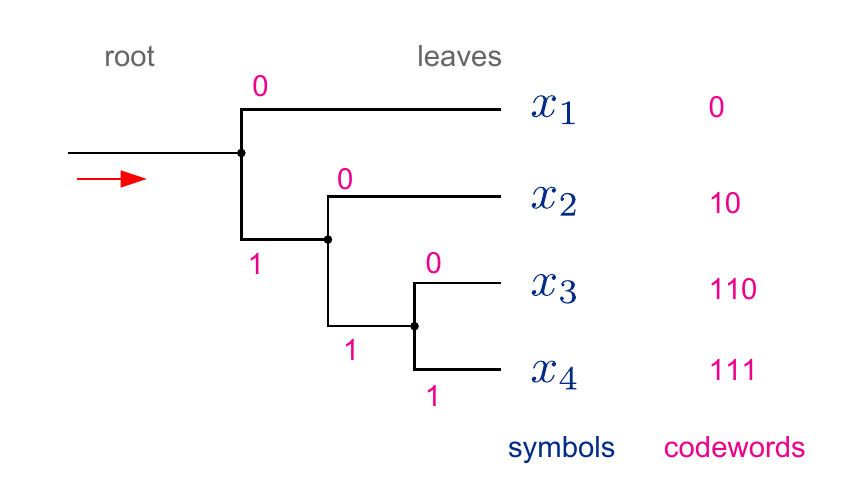
\includegraphics[width=0.5\textwidth]{./img/grundl_quellencod_codebaum.png}
	\caption{Codebaum \protect\cite{NT2}}
	\label{fig:grundl_quellencod_codebaum}
\end{figure}
\end{bem}

\subsubsection{Huffman Codierung}
\begin{bem}
	Ziel der Huffman-Codierung ist es einen minimierten und präfixfreien Code zu erzeugen. 
	Mathematisch ausgedrückt lautet die Bedingung also:
	\begin{equation}
		\overbar{m} = \sum\limits_{i=1}^N P_i \cdot m_i \overset{!}{=} \min\limits_{\forall \lbrace m_1, ..., m_N\rbrace }
	\end{equation}
	Damit folgt $P_i \uparrow \; \Rightarrow m_i \downarrow$ und $P_i \downarrow \; \Rightarrow m_i \uparrow$. Der Ablauft der Huffman-Codierung ist wie folgt:
	\begin{description}
		\item[1) ] $x_i$ nach fallenden $P_i$ ordnen.
		\item[2) ] Aus $X_N$ und $X_{N-1}$ neues Symbol mit $P_n + P_{N-1}$ bilden.
		\item[3) ] Schritt 1) und Schritt 2) wiederholen, bis nur noch ein Symbol übrig ist.
		\item[4) ] Knoten des Baums jeweils $0$ und $1$ zuordnen. Die Zuordnung ist beliebig, es macht aber Sinn ein System einzuführen. Empfehlung aus der Vorlesung: $0$ für größere und $1$ für kleinere Wahrscheinlichkeit.
	\end{description}
		\begin{figure}[H] 
		\centering
		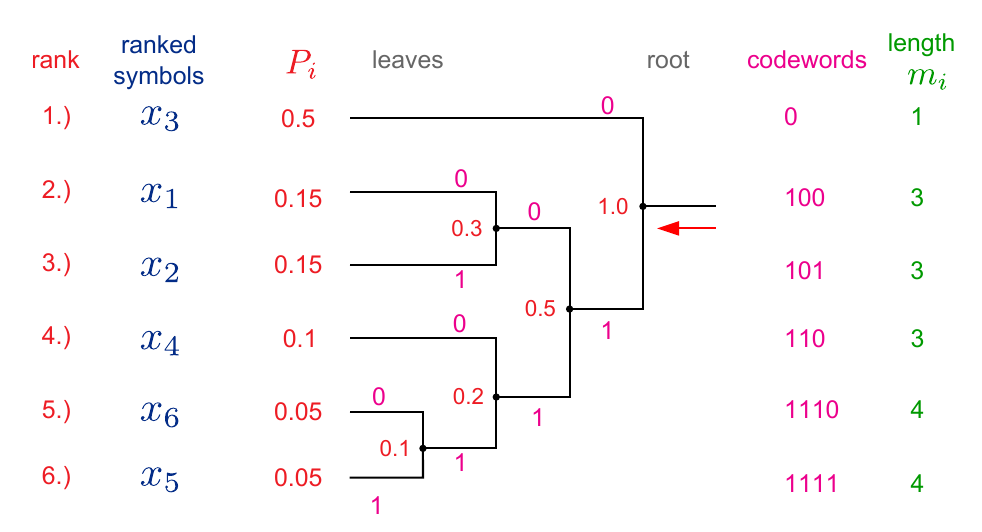
\includegraphics[width=0.5\textwidth]{./img/grundl_quellencod_huffman.png}
		\caption{Huffman Codierung \protect\cite{NT2}}
		\label{fig:grundl_quellencod_huffman}
	\end{figure}
\end{bem}

\subsection{Vergleich von Wahrscheinlichkeitsbetrachtungen}
\subsubsection{Einzelwahrscheinlichkeit}
$P[A]$ gibt an, wie wahrscheinlich es ist, dass $A$ eintritt.

\subsubsection{Verbundwahrscheinlichkeit}
$P[A,B]$ gibt an, wie wahrscheinlich es ist, dass $A$ und $B$ zusammen eintreten.
\formTab{Satz von Bayes}{P[x_i, y_j] = P[y_j|x_i] \cdot P[x_i] = P[x_i|y_j] \cdot P[y_j]}

\subsubsection{Übergangswahrscheinlichkeit/Bedingte Wahrscheinlichkeit}
$P[B|A]$ gibt an, wie wahrscheinlich es ist, dass $B$ eintritt wenn $A$ bereits eingetreten ist.
\formTab{Es gilt}{\sum\limits_{j=1}^N P[y_j|x_i] = 1 \quad \text{für } i = const}
\formTab{Bestimmung von $P[y_j]$}{P[y_j] = \sum\limits_{i=1}^M P[x_i, y_j] = \sum\limits_{i=1}^M P[y_j|x_i]\cdot P[x_i]}

\subsubsection{Übergangsmatrix}
Die Übergangsmatrix definiert sich als
\begin{align*}
T &= (P[y_j|x_i])_{M\times N} = (P_{ij})_{M\times N}
	= \left( \begin{array}{c c c}
			P[y_1 | x_1] & \dots & P[y_N | x_1]\\ 
			\vdots & \ddots & \vdots \\
			P[y_1|x_M] & \dots & P[y_N|x_M]
			\end{array} \right) \nonumber \\
			&=\left( \begin{array}{c c c}
			P_{11} & \dots & P_{1N}\\ 
			\vdots & \ddots & \vdots \\
			P_{M1} & \dots & P_{MN}
			\end{array} \right)
\end{align*}

\subsubsection{Binärkanal (BC)}
\begin{figure}[H] 
		\centering
		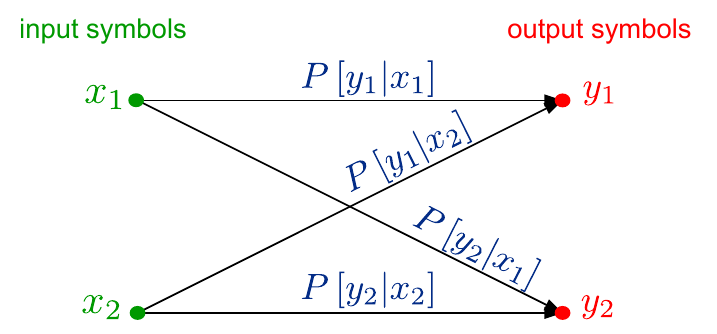
\includegraphics[width=0.5\textwidth]{./img/grundl_kanalmod_bc.png}
		\caption{Binärkanal (BC) \protect\cite{NT2}}
		\label{fig:grundl_kanalmod_bc}
\end{figure}
Es gilt $input\;M=2$ und $output\;N=2$. Ferner ist die Übergangsmatrix gegeben mit
\begin{equation}
	T = \left( \begin{array}{c c}
	P_{11} & P_{12} \\
	P_{21} & P_{22}	
	\end{array} \right)
\end{equation}

\formTab{Fehler}{P_{err} = P[x_1,y_2]+P[x_2,y_1] \formTnQ=P[x_1] \cdot P[y_2|x_1] + P[x_2] \cdot P[y_1|x_2] \formTnQ = P_1 P_{12}+P_2 P_{21}}

\subsubsection{Symmetrischer Binärkanal (BSC)}
\begin{figure}[H] 
		\centering
		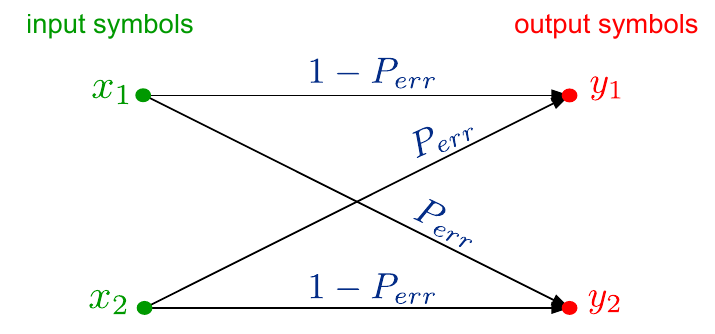
\includegraphics[width=0.5\textwidth]{./img/grundl_kanalmod_bsc.png}
		\caption{Symmetrischer Binärkanal (BSC) \protect\cite{NT2}}
		\label{fig:grundl_kanalmod_bsc}
\end{figure}
Es gilt $P_{12} = P_{21} = P_{err}$. Die Übergangsmatrix ist gegeben durch
\begin{equation}
	T = \left( \begin{array}{c c}
	1-P_{err} & P_{err} \\
	P_{err} & 1-P_{err}	
	\end{array} \right)
\end{equation}

Mit $P_2 = 1-P_1$ ergibt sich 
\formTab{Fehler}{P_{err, BSC} = P_{err} P_1 + P_{err} P_2 = P_{err}(P_1 + 1 - P_1) \formTnQQQ = P_{err}}

\subsubsection{Binärer Verlustkanal (BEC)}
\begin{figure}[H] 
		\centering
		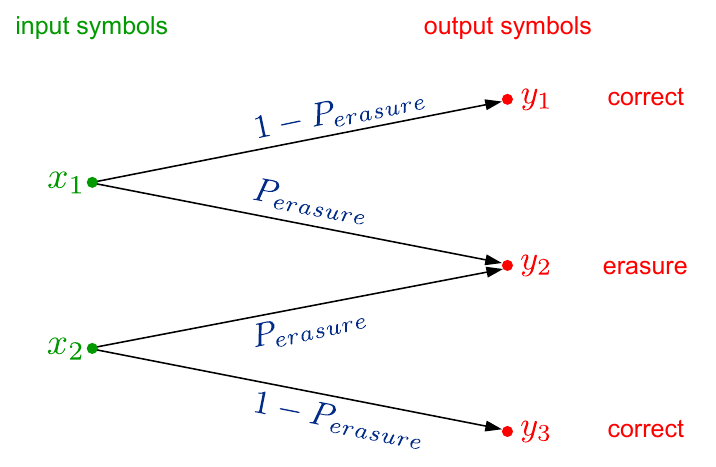
\includegraphics[width=0.5\textwidth]{./img/grundl_kanalmod_bec.png}
		\caption{Binärer Verlustkanal (BEC) \protect\cite{NT2}}
		\label{fig:grundl_kanalmod_bec}
\end{figure}
Die Übergangsmatrix ergibt sich zu
\begin{equation}
	T = \left( \begin{array}{c c c}
	1-P_{erasure} & P_{erasure} & 0 \\
	0 & P_{erasure} & 1-P_{erasure}	
	\end{array} \right)
\end{equation}


\subsection{Kanalkapazität}
\subsubsection{Wechselseitige Information/Transinformation/mutual information}
\formTabL{Informationsgehalt a priori}{I(x_i) = \ld\left(\fracd{1}{P[x_i]} \right)}{grundl_kanalkap_apri}
\formTabL{Informationsgehalt posteriori}{I(x_i) = \ld\left(\fracd{1}{P[x_i|y_j]} \right)}{grundl_kanalkap_ppri}
Differenzbildung aus \eqref{eq:grundl_kanalkap_apri} und \eqref{eq:grundl_kanalkap_ppri} liefert die wechselseitige Information also den Informationsgewinn:
\formTabL{Wechselseitige Information}{I(x_i; y_j) = \ld\left(\frac{1}{P[X=x_i]}\right) - \ld\left(\frac{1}{P[X=x_i|Y=y_j]} \right) \formTnQQQ= \ld\left(\fracd{P[X=x_i|Y=y_j]}{P[X=x_i]}\right)}{grundl_kanalkap_wechsel_a}

\formTab{Rausch- und störungsfreie}{I(X;Y) = H(X)}
\formTab{Vollständig gestört}{I(X;Y) = 0}
\formTab{Symmetrie}{I(x_i; y_j) = I(y_j, x_i)}
Bestimmungsgleichungen für $I(x_i; y_j)$:
\begin{align}
	P[x_i, y_j] &= P[y_j|x_i]\cdot P[x_i] \nonumber\\ 
	I(x_i; y-J) &= \ld\left(\frac{1}{P[x_i]} \cdot P[x_i|y_j] \right)\nonumber \\
	P[x_i|y_j] \cdot P[y_j] &= P[y_j|x_i] \cdot P[x_i] = P[x_i,y_j] \nonumber\\
	P[y_j] &= \sum\limits_{i=1;\; j\;fest}^M P[x_i, y_j] = \sum\limits_{i=1; \; j\;fest}^M P[y_j, x_i] \cdot P[x_i] \nonumber\\
	\Rightarrow I(x_i; y_j) &= f(P[x_i], P[y_j|x_i])
\end{align}

\subsubsection{Mittlere wechselseitige Information}
\formTabL{Mittlere wechselseitige Information}{I(X;Y) = \sum\limits_{i=1}^M \sum\limits_{j=1}^M P[X=x_i, Y=y_j] \cdot \ld\left(\frac{P[X=x_i|Y=y_j]}{P[X=x_i]}\right) \formTnQ = \sum\limits_{i=1}^M \sum\limits_{j=1}^M P[X=x_i, Y=y_j] \cdot I(x_i; y_j) \formTnQ = \sum\limits_{i=1}^M \sum\limits_{j=1}^M P[X=x_i, Y=y_j]   \cdot \ld\left(\frac{P[Y=y_j|X=x_i]}{P[Y=y_j]}\right) \formTnQ = I(Y;X)}    {grundl_kanalkap_wechsel_rel}

\subsubsection{Kanalkapazität}
\formTabL{Kanalkap. a)}{C = \max\limits_{\forall P[x_i]} I(X;Y) = I^* (X;Y)}{grundl_kanalkap_kanalkap_a}
\formTabL{Kanalkap. b)}{C= f(P[y_j|x_i)}{grundl_kanalkap_kanalkap_b}
\formTabL{Kanalkap. BSC}{C_{BSC}(P_{err}) = 1-H_b(P_{err}) \formTnQQQ \text{ für }P[x_1] = P[x_2] = \frac{1}{2}}{grundl_kanalkap_kanalkap_bsc}
\formTab{Entropie Binärkanal}{H_b = -P_{err}\cdot \ld(P_{err}) - (1-P_{err}) \cdot \ld(1-P_{err}) \formTnQQQ = p \cdot \ld\left( \frac{1}{p}\right) + (1-p) \cdot \ld\left(\frac{1}{1-p}\right)}

\subsection{AWGN-Kanal (\underline{A}dditive \underline{W}hite \underline{G}aussian \underline{N}oise)}
\formTabL{AWGN-Signal}{y_k = x_k + n_k \qquad y_k \in \R ,\; x_k \in \lbrace -1, 1 \rbrace ,\; n_k \in \R}{grundl_awgn_a}
\formTabL{Noise}{n_k \sim \bm{N}(0, \sigma^2)}{grundl_awgn_b}
\formTabL{Gauss Funktion a)}{p_n(\xi) = \fracd{1}{\sqrt{2 \pi \sigma}}\cdot e^{-\fracd{1}{2 \sigma^2}\xi^2}}{grundl_awgn_gauss_a}
\formTabL{Gauss Funktion b)}{\int\limits_{-\infty}^\infty p_n(\xi)\; d\xi = 1}{grundl_awgn_gauss_b}
\formTab{Varianz der Gauss Funktion}{\sigma^2 = \frac{1}{N}\sum\limits_{i=1}^N (n_i-\mu^2) \quad \text{meist }\mu = 0}

\subsubsection{Signal Noise Ratio (SNR)}
\formTabL{Signal-Noise-Ratio}{SNR = \fracd{E_s}{\sigma^ 2} = \fracd{P_s}{P_n} = \fracd{E[|x_k|^2}{E[|n_k|^2} = [Q^{-1}(P_{err})]^2}{grundl_awgn_snr_a}
\formTabL{Signalleistung}{P_s = E[|x_k|^2]}{grundl_awgn_snr_sign}
\formTabL{Rauschleistung}{P_n = E[|n_k|^2] = \sigma^2}{grundl_awgn_snr_raus}
\formTabL{Q-Funktion}{Q(x) = \fracd{1}{\sqrt{2\pi}}\int\limits_x^\infty e^{-\frac{1}{2} \xi^2} d\xi = \fracd{1}{2}(1-erf(\frac{1}{\sqrt{2}})}{grundl_awgn_gauss_q}

\subsubsection{Sonderfall Hard Decision}
\formTabL{Fehler}{P_{err} = Q(\sqrt{SNR}) \qquad ,\;mit\;SNR = \frac{1}{\sigma^2}}{grundl_awgn_gauss_fehler}

\subsubsection{Kapazität}
\formTabL{Kapazität BSC}{C_{BSC}(SNR) = 1-H_b(\underbrace{Q(\sqrt{SNR}}_{=P_{err}}) \formTnQQQ = 1 - H_b(P_{err})}{grundl_awgn_gauss_kap_bsc}
\formTabL{Kapazität AWGN}{C_{AWGN}(SNR) = \frac{1}{2} \log_2(1+SNR)}{grundl_awgn_gauss_kap_awgn}

\subsection{Kanalcodierung}
Der Satz von Shannon gibt an ab wann eine fehlerfreie Übertragung prinzipiell möglich ist.
\formTabL{Satz von Shannon}{H(X) \leq I(X;Y)}{grundl_kanalc_shannon}
\formTabL{Kanalcodierrate}{R_C = \frac{K}{N}}{grundl_kanalc_rate}
Wobei $K$ der Bitlänge der uncodierten Nachricht und $N$ der Bitlänge des Codewortes entsprechen.
\formTab{Maximale Bitfehler damit Fehlerkorrektur möglich ist}{n_{err} \leq \left\lfloor \fracd{d_{min} -1}{2}\right\rfloor}
Meis wird für die Kanalcodierung eine Codewortmatrix $CWT$ mit Codiervorschrift $\bm{c}$ aufgestellt:
\begin{align}
	CWT  &= \left( \begin{array}{c c c | c c c}
		\colGreen{0} & \colGreen{0} & \colGreen{0} & \colGreen{0} & \colGreen{0} & \colGreen{0} \\
		0 & 0 & 1 & 0 & 1 & 1 \\
		0 & 1 & 0 & 1 & 0 & 1 \\
		0 & 1 & 1 & 1 & 1 & 0 \\
		1 & 0 & 0 & 1 & 1 & 0 \\
		1 & 0 & 1 & 1 & 0 & 1 \\
		\colBlue{1} & \colBlue{1} & \colBlue{0} & \colBlue{0} & \colBlue{1} & \colBlue{1} \\
		\colRed{1} & \colRed{1} & \colRed{1} & 0 & 0 & 0 \\	
	\end{array} \right) \\
	\bm{c}  &= \left( \bm{u}, u_1 \oplus u_2, u_1 \oplus u_3, u_2 \oplus u_3 \right)
\end{align}

\begin{flalign}
	&\colGreen{u(0,0,0)} = 000\;000&\\
	&\colBlue{N} = 6 &\\
	&\colRed{K} = 3&%
\end{flalign}
wobei die linke Spalte alle möglichen Bitkombinationen für die uncodierte Nachricht und die rechte Spalte die kontrollierte Redundanz mit Codewort-Vorschrift enthält. Eine komplette Zeile über beide Spalten entspricht einem Codewort (in grün dargestellt) für die entsprechende uncodierte Nachricht. Anhang der Anzahl der Bitstellen einer Zeile der linken Spalte (in rot dargestellt) lässt sich $K$ ablesen. Anhand der Bitstellen einer gesamtem Zeile (blau dargestellt) lässt sich $N$ ablesen. 

\formTab{Energie pro bit}{E_b = \frac{1}{R_C} \cdot E_s}
\formTab{Normierter Signal-Rauschabstand}{SNR_b = \frac{1}{R_C} \cdot SNR_s = \fracd{E_b}{\sigma^2} = \fracd{1}{C \frac{E_s}{\sigma^2}}\fracd{E_s}{\sigma^2}}
\formTab{Signal-Rauschabstand}{SNR = SNR_s = \frac{E_s}{\sigma^2}}

\subsubsection{Hamming-Distanz}
\formTab{Hamming-Distanz}{h(c_i, c_h) = \sum\limits_{i=1}^N c_{1, i} \oplus c_{2,i}}
\formTab{Minimale Hamming-Distanz}{h_{min} = d_{min} = \min\limits_{\forall i,j (i\neq j)} \left( h(c_i, c_j)\right)}
\begin{bem}
	Die minimale Hamming Distanz lässt sich auch einfacher bestimmen. Dazu wird das Codewort mit den wenigsten $1$en gesucht. Die Anzahl der Bitstellen die $1$wertig sind entsprechen der minimalen Hamming-Distanz.
\end{bem}